\chapter{Deep Neural Networks}
\label{chap:dnn}
\section{Introduction}
The major Problem in \textit{Machine Learning} is that in most of real world applications, many factors of variation influence every single piece of data. Most of real world applications require us to disentangle these factors of variation in data and discard the ones which we don't care about. But it can be very difficult to extract these high level abstract features from raw data obtained. \textit{Deep learning} aims solves this problem in representation learning by introducing representations that are expressed in terms of other, simpler representations.

According to \cite{deng2014deep}, \textit{``Deep learning is a set of algorithms in machine learning that attempt to model high-level abstractions in data by using model architectures composed of multiple non-linear transformations"}.They are also called hierarchical learning or deep structured learning. 

Most of the successful deep learning methods uses principles of \textit{Artificial Neural Networks (ANN)}. Different deep learning architectures like Deep Belief Networks (DBN) and Convolutional Neural Networks (CNNs) produced state-of-the-art results in different fields like image recognition, natural language processing and automatic speech recognition.

In this chapter we fist introduces Deep Neural Network and its bacic concepts in \ref{sec:dnn:dnn}. Later we briefly discuss common DNN architecture like \textit{CNNs, DBN, etc}.

\section{Deep Neural Network}
\label{sec:dnn:dnn}
Artificial neural networks are family of statistical learning models inspired by the \textit{biological model of 1959 (by Nobel prize winners T.Wiesel and D.~H.~Hubel)}. A \textit{DNN (Deep Neural Network)} can be considered as a form of Artificial Neural Network, with multiple hidden layers. 


\subsection{Motivations for Deep Architectures}
The Major motivations for deep architectures are the following:

\subsubsection{Deep architecture of Brain}
One of major motivation of Deep Architectures is deep structure of brain. For example, study of visual cortex, shows areas which contains representation of the input, and how signals are flowing from an area to the next. Each level defines different level of abstractions. And in higher level, more abstract features represented in terms of the lower-level features. Moreover, representation in brain is neither local nor dense distributed. These representation in brain are sparse (only 1\% of neurons are simultaneously active). 

\subsubsection{Insufficient depth can hurt}
According to complexity theory of circuit, compared to shallow architectures, deep architectures are more efficient in terms of number of parameters and computational elements for representing functions\citep{bengio2007scaling}. Haastad found that a function (of $n$ inputs) which can be efficiently represented with $O(n)$ nodes with a depth $d$, requires an ($O(2^n)$) nodes if depth is $d-1$. \citep{bengio2007greedy}

\subsubsection{Cognitive processes seem deep}
If you consider process of perceiving by humans, we always organize ideas and concepts hierarchically. Humans first learns simple concepts and then composes these concepts for representing more abstract ones. 


\subsection{General Deep Network Framework}
As discussed in Section \ref{sec:dnn:dnn} Deep Neural Network can be considered as Multilayer perceptron with many hidden layers. Standard learning strategy of MLP contains following steps:
\begin{itemize}
\item The weights of Neural network is initialized by random values
\item Apply gradient descent using back-propagation (BP) algorithm.
\end{itemize}
But Apart from few exceptions, researchers soon found out that an MLP of more
than two hidden layers often failed \cite{bengio2007greedy} due to a well-known fact that the MLP learning involves an extremely difficult non-convex optimization problem and a gradient-based local search used in the BP algorithm easily gets stuck in local minimum.

So For training Deep Network, \citet{hinton2006reducing} proposed a greedy layer-wise training algorithm. It contain following major steps:
\begin{itemize}
\item \textsc{Pretraining}: Each layer is trained in a greedy way. This is a unsupervised learning at each layer so that information from the input is preserved and factors of variation in data is untangled. This act as initialization step. Hence, instead of doing a random initialization, we perform careful initialization and reduce chance of getting stuck on local minima.
\item \textsc{Finetuning}: Then network is fine-tuned with respect to the ultimate aim which may be classification or regression task.
\end{itemize}

\section{Deep Belief Networks}
\citet{hinton2006reducing} introduced \emph{Deep Belief Networks (DBN)} which is a stacking of \emph{Restricted Boltzmann Machines (RBMs)}. Deep Belief Networks can be trained in a greedy manner\cite{hinton2006reducing}. Deep Belief Network is graphical model which tries to represent data into a deep hierarchical features. First, an unsupervised training is performed on each layer (RBM) in a greedy manner. Then fine-tune network based on a supervised training criterion.\\
\begin{figure}[!ht]
\centering
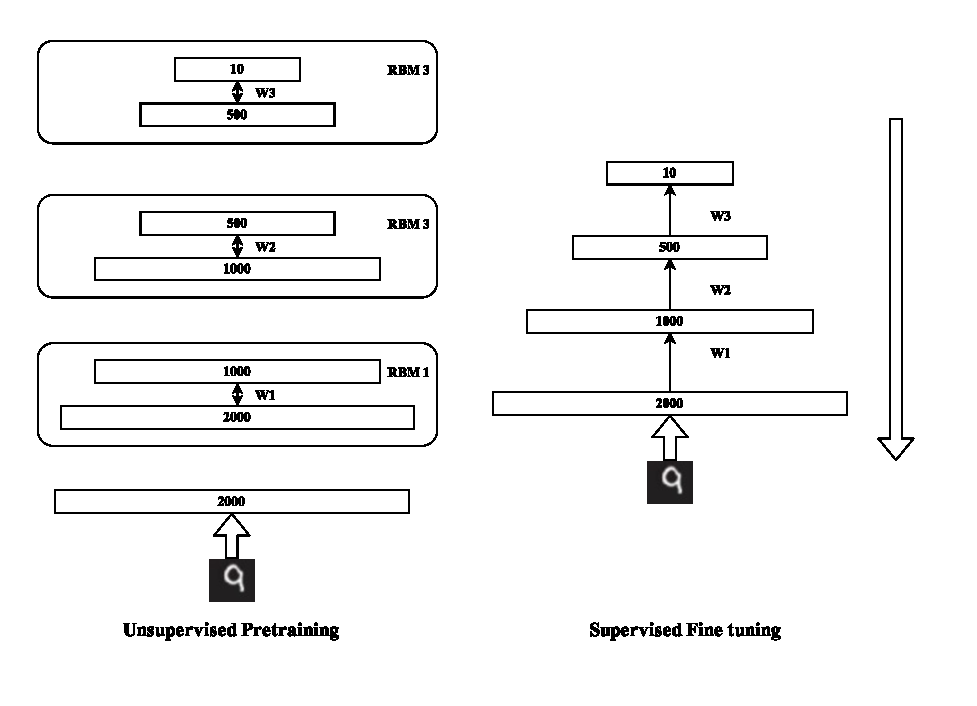
\includegraphics[width=1\textwidth]{./imgs/RBM_Train.eps} 
\caption{Training of DBN}
\end{figure}

Restricted Boltzmann Machine (RBM) is an energy-based model. A graphical representation of an RBM is shown in figure. \ref{fig:rbm_layer}.

\begin{figure}[!ht]
  \centering
  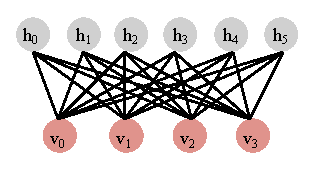
\includegraphics[width=0.5\textwidth]{./imgs/rbm.eps}
  \caption{A Restricted Boltzmann Machine Layer}
  \label{fig:rbm_layer}
\end{figure}%

Like every other energy based models, RBM also has energy for every possible configuration of parameters. The Energy function of RBM, $E(v,h)$ is defined as: 
$$E(v,h) = - b'v - c'h - h'Wv$$
where $W$ is weights between hidden and visible units and $b$ and $c$ are the bias of the visible($v$) and hidden layers($h$) respectively. Like other Energy based models, RBM also uses free energy (inspired from physics), which is defined as
$$\mathcal{F}(v) = -log \sum_{h}{e^{-(E(v,h))}} $$
$$\mathcal{F}(v) = - b'v - \sum_i \log \sum_{h_i} e^{h_i (c_i + W_i v)}$$

Since hidden nodes and visible nodes are conditionally independent and binary units (where $v_j \& h_i \in \{0,1\}$), we have 
%\begin{equation} 
\begin{align}
p(h|v) &= \prod_i p(h_i|v) \\
p(v|h) &= \prod_j p(v_j|h) \\
P(h_i=1|v) &= sigm(c_i + W_i v) \label{eq:rbm_layers_prob1} \\
P(v_j=1|h) &= sigm(b_j + W'_j h) \label{eq:rbm_layers_prob2} 
\end{align}

And hence free energy becomes 
$$\mathcal{F}(v)= - b'v - \sum_i \log(1 + e^{(c_i + W_i v)})$$ %\label{eq:rbm_freeE}
Probability distributions over visible vectors can be defined in terms of the free energy.
%p(v) = \frac {e^{-E(v)}} {Z} \text{ with } Z = \sum_v e^{-E(v)} \\
\begin{align*}
P(v) = \frac{e^{-\mathcal{F}(v)}}{Z} \text{, where } Z=\sum_v e^{-\mathcal{F}(v)}.
\end{align*}
Restricted Boltzmann machines are trained to maximize the product of probabilities assigned to some training set. It is almost impossible to determine this gradient, because it requires to compute $E_P[\frac{\partial \mathcal{F}(v)} {\partial \theta} ]$. This is an expectation over all attainable configurations of input ($v$). \cite{hinton2010practical}

A faster learning algorithm was proposed by Hinton \cite{hinton2002training,hinton2006reducing,hinton2010practical}. It starts by assigning values in a training vector as the states of the visible nodes. Then the states of all hidden nodes are computed using equation \ref{eq:rbm_layers_prob1}. After binary states computed for the hidden units, each $v_i$ is made $1$ with a probability calculated by equation \ref{eq:rbm_layers_prob2} to produce a \textit{reconstruction}. This process is repeated for $k$ steps to produce $v'= v^{(k)}$ and $h' = h^{(k)}$. 

\begin{figure}[ht]
\centering
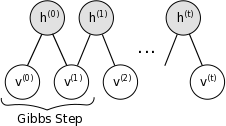
\includegraphics[width=0.3\textwidth]{./imgs/markov_chain.png}
\caption[Markov chain of training RBM layer]{Markov chain, that uses alternating Gibbs sampling for training RBM layer. $(v^{(t)}, h^{(t)})$ become accurate samples of $p(v,h)$ when $t \rightarrow \infty$}
\label{fig:rbmmarkovChain}
\end{figure}

The change in the weights is given by
$$ \Delta W = \eta ({vh^\mathsf{T}}_{data} - {v'h'^{\mathsf{T}}}_{recon}). $$
where $\eta$ is learning rate. Outer product $vh^\mathsf{T}$ is called as the positive gradient and that of of $v'$ and $h'$ as negative gradient. The Adaption of biases of hidden and visible layer is done by a similar learning method that uses the states of individual nodes. This process is called \textbf{Contrastive Divergence (CD-k)}. In practice, $k=1$ has been shown to work exceptionally well \cite{hinton2010practical}.

\section{Stacked Denoising Auto-encoders}
\citet{vincent2010stacked} introduced the \emph{Stacked Denoising Auto-encoder (SdA)} which is a modified version of the stacked auto-encoder. The Stacked Denoising Auto-encoder (SdA) is formed by stacking of denoising auto-encoders so that input of each layer ($dA_i$) is the hidden representation produced by the layer below ($dA_{i-1}$). The pre-training of SdA is performed on one layer at a time. That is, every layer is trained independently so that the reconstruction error with respect to input of current layer (output of the previous denoising auto-encoder layer) is minimized. Once this unsupervised \textit{pre-training} is completed on all layers, the network undergoes a another stage of training called supervised \textit{fine-tuning} where aim is to make prediction error of the supervised task minimum.

The idea of auto-encoders has been part of the landscape of neural networks for decades. The aim auto-encoder is to encode the input $x$ into some latent representation $y = f(x)$ so that the input can be regenerated from the latent representation. The auto-encoder has two components: the encoder $f:x \rightarrow y$ and the decoder $g:y\rightarrow z$. The reconstruction error of Auto-encoder can be computed in different ways. Appropriate error measure is determined by the distributional assumptions on the input. More commonly used are:
\begin{itemize}
\item Squared error.
$$ L(\mathbf{x} \mathbf{z}) = || \mathbf{x} - \mathbf{z} ||^2$$
\item If the inputs can be considered as binomial probabilities or inputs are binary, then we can use cross-entropy between input and reconstruction as Error Measure.
$$L(\mathbf{x}, \mathbf{z}) = - \sum^d_{k=1}[\mathbf{x}_k \log \mathbf{z}_k + (1 - \mathbf{x}_k)\log(1 - \mathbf{z}_k)]$$
\end{itemize}

The principle behind \emph{denoising auto-encoders (dA)} is that, \textit{in order to force the hidden layer to discover more robust features and prevent it from simply learning the identity, the auto-encoder is trained to reconstruct the input from a corrupted version of it} \cite{vincent2008extracting}. The denoising auto-encoder can be viewed as a stochastic version of the auto-encoder. The stochastic corruption process randomly make few of nodes in the inputs layer to $0$ with a probability (called as corruption rate). Then auto-encoder tries to predict the original vector from the it's corrupted vectors. Hence, \textit{able to predict any subset of variables from the rest} is a adequate condition for effectively capturing the joint distribution between a set of variables.

\begin{figure}[ht]
\centering
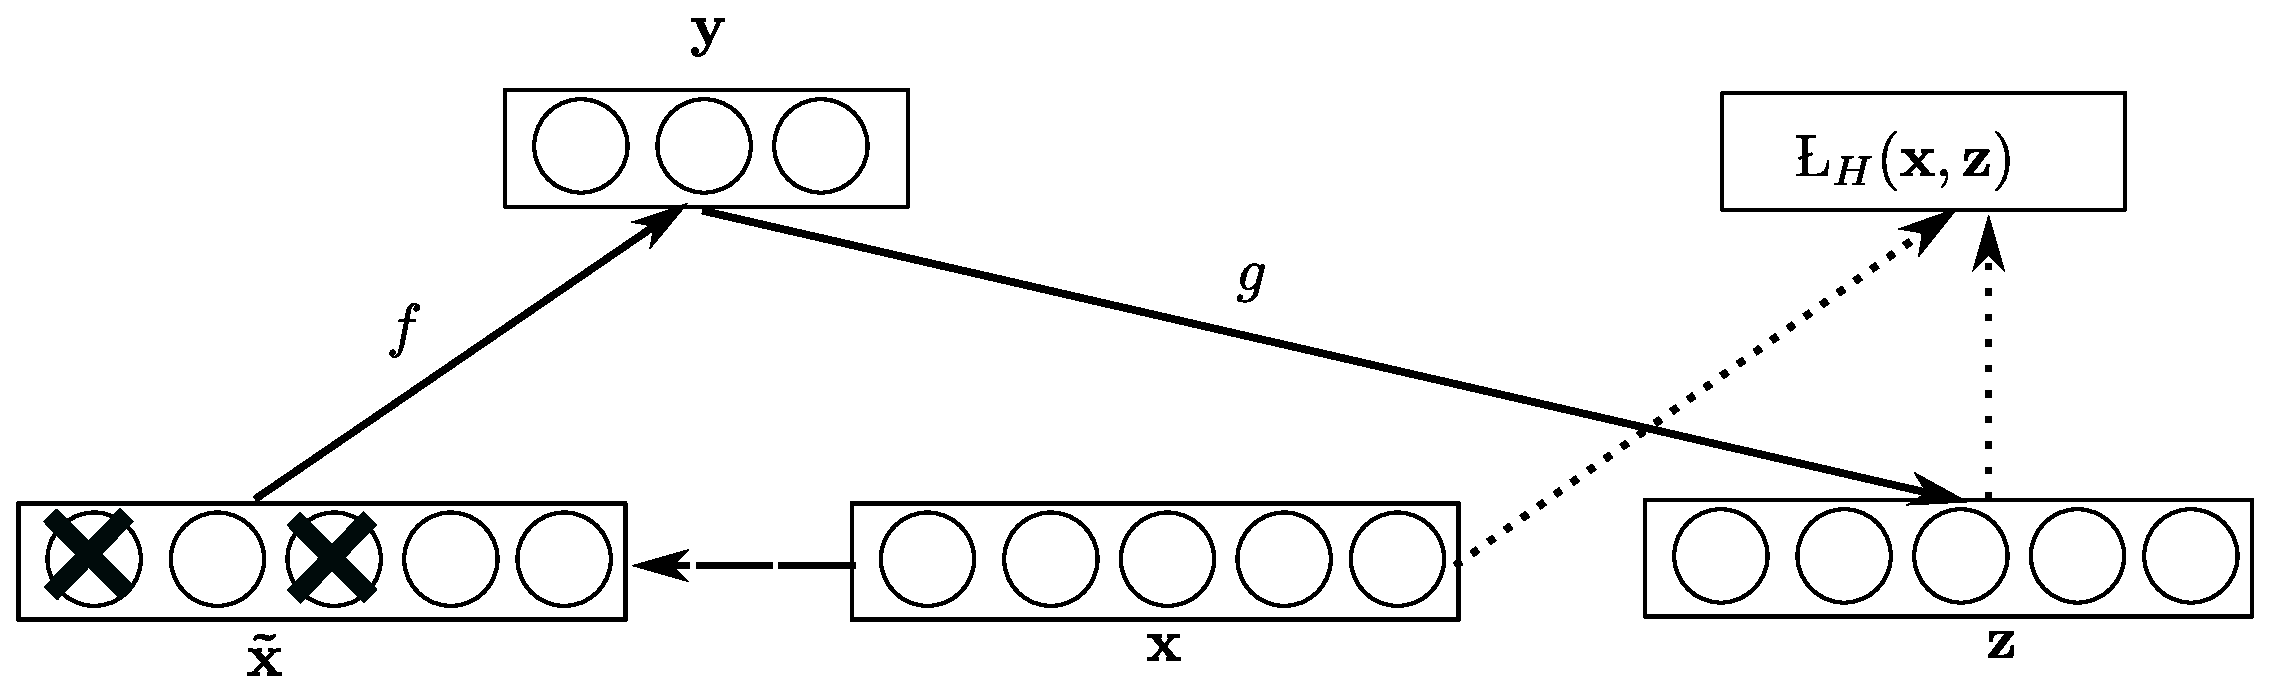
\includegraphics[width=0.8\textwidth]{./imgs/sda.eps}
\caption[The denoising auto-encoder architecture]{The denoising auto-encoder architecture. $\mathbf{\tilde{x}}$ is a corrupted version of a train vector $\mathbf{x}$. The auto-encoder maps (encodes) $\mathbf{\tilde{x}}$ to $\mathbf{y}$ ($\mathbf{y} = f(\mathbf{\tilde{x}})$). Then auto-encoder attempts to reconstruct $\mathbf{x}$ , resulting $ \mathbf{z} = g(\mathbf{y}) $. Reconstruction error is measured by loss $L_{H}(\mathbf{x},\mathbf{z})$. }
\label{fig:sdaChain}
\end{figure}

\section{Convolutional Neural Networks}
\emph{Convolutional Neural Network (CNN)} is a variant of Multilayer perceptron and inspired by biological processes (From complex arrangement of cells in the cat's visual cortex). Convolutional Neural Networks are designed to use less amount of preprocessing \cite{lecun1998gradient}. It was Introduced by Fukushima in 1980 and later improved by \citet{lecun1998gradient}. CNNs are widely used as image \& video recognition model. CNNs make use of local receptive fields, shared weights and spatial sub-sampling to ensure some degree of shift, scale and distortion invariant.

\noindent Two key idea of Convolutional Neural Network are
\begin{itemize}
\item \textsc{Sparse Connectivity:} The inputs to hidden nodes in layer $m$ are from a subset of nodes in layer $m-1$, which have spatially contiguous receptive fields. This create a receptive field behavior and hence ensure that filters produce strong response to a spatially local pattern in input.


\item \textsc{Shared Weights:} Each filter $h_i$ of CNN is replicated. These replicated filters share the same weight matrix and bias vector. This replication of weights not only reduces the number of parameters to be estimated but also make CNN to learn position invariant feature detection.
\end{itemize}

\begin{figure}[!ht]
\centering
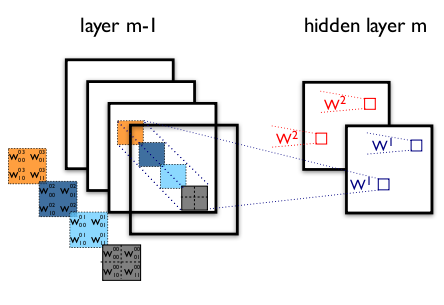
\includegraphics[width=0.6\textwidth]{./imgs/convolution.png} 
\caption[convolutional layer explained]{An example convolutional layer.  There are four feature maps in ${(m-1)}^{th}$ layer and two (represented by $h^0$ and $h^1$) in next ($m$). The blue and red squares denotes pixel values in feature maps ($h^0$ and $h^1$) in the $m^{th}$ layer. These pixels are computed from $(m-1)^{th}$ layer pixels that falls within the $2\times2$ receptive field of corresponding kernel (represented as colored rectangles).}
\label{fig:cnn_layer}
\end{figure}


\noindent CNNs tries to capture high level feature of input images using following operations:
\begin{itemize}
\item \textsc{Convolution}: Most important operation of CNN is convolution. A \textit{feature map} is obtained by convolution of the input image with a linear filter and then applying a non-linear function. 
$$h^k_{ij} = fn( (W^k * x)_{ij} + b_k ).$$
Since this linear filter is applying repeatedly, the resulting connectivity act as a series of overlapping receptive fields \cite{KarpathyCVPR14}.
\item \textsc{Sub Sampling}: Sub-sampling refers to reducing the overall size of a signal. The most commonly used subsampling method is \textit{max pooling}. Max pooling divides the input feature map into a collection of sub-regions which are non-overlapping, and emits the maximum value in each such sub-region. It help in reduction of computation for higher layers. Moreover, it provides some form of translation invariance. 
\end{itemize}

\begin{figure}[!ht]
\centering
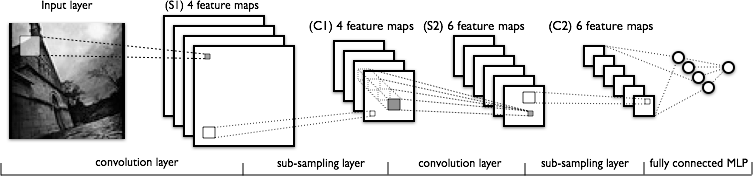
\includegraphics[width=0.9\textwidth]{./imgs/cnn1.png} 
\caption[An example of a convolutional neural network]{A typical example of a CNN \footnote{From site: http://white.stanford.edu/}. }
\label{fig:cnn}
\end{figure}

Typically, Convolutional Neural Networks consists of a number of convolutional and subsampling layers optionally followed by fully connected layers (MLP). Some times we can use SVM instead of MLP. The input to a convolutional layer is a $m \times n \times r$ image where $m$ is the height and width of the image and $r$ is the number of channels (eg: 3 for RGB)/input feature maps. 

\subsection{3D Convolutional Neural Networks}
3D Convolutional Neural Networks extracts features from both the spatial and the temporal domain by performing 3D convolutions, hence capturing the motion information from multiple adjacent frames.\cite{ji20133d} The value at $(p, q, r)$ on the $j^{th}$ feature map (in the $i^th$ layer) is given by
$$v^{pqr}_{ij} = \tanh(b_{ij}+\sum_{m} \sum_{x=0}^{X_i-1} \sum_{y=0}^{Y_i-1} \sum_{z=0}^{Z_i-1} w^{xyz}_{ijm} v^{(p+x)(q+y)(r+z)}_{(i−1)m}) $$
where $X_i \times Y_i \times Z_i$ is the size (height, width and depth along along the temporal
dimension) of the 3D kernel and $w^{xyz}_{ijm}$ is the cost of the 3D kernel connected to the $m^{th}$ feature map in the $i^{th}$ layer. Similarly Pooling/Sub-sampling is done in both spatial and temporal domain.

\section{Summary}
Deep learning algorithms attempts learn model high-level abstractions in data by help of multiple non-linear transformations. Deep Neural Networks is basically Artificial Neural Network with multiple hidden layers between input and output. Major characteristics of Deep Learning are:
\begin{itemize}
\item They are usually Multilayered and Hierarchical.
\item They contains Multiple non-linear transformations 
\item They act as a feature extractors, they tries to high level abstract features from raw data.
\end{itemize}

Most of DNNs have greedy layer-wise training algorithm (pretraining) for initialization weights and followed by supervised fine-tuning.
 
Deep Belief Network is made of stacking of RBM layers. RBM attempts to reduce Free energy of network, and trained by Contrastive Divergence.
 
Denoising Auto-encodes can be stacked to form SdA. The aim of denoising Auto-encodes to predict the original data from the it's corrupted version.

Convolutional Neural Network contains a series of Convolution and sub sampling layers and optionally fully connected layer. CNN uses spatial sub-sampling and shared weights to provide some degree of freedom from shift, scale and distortion of input.
